\documentclass{config/apuntes}

\title{Algoritmos en Bioinformática}
\author{Sandra Mingo Ramírez}
\date{2024/25}
\acronym{ALGBIO}

\usepackage[all]{nowidow}
\usepackage{listing}
\usepackage{color}
\usepackage{tabularx}
\usepackage{multirow}
\usepackage{makecell}
\usepackage{amsmath}
\usepackage{array}

\definecolor{dkgreen}{rgb}{0,0.6,0}
\definecolor{gray}{rgb}{0.5,0.5,0.5}
\definecolor{mauve}{rgb}{0.58,0,0.82}

\lstset{
  language=Python,
  frame=tb,
  aboveskip=3mm,
  belowskip=3mm,
  showstringspaces=false,
  columns=flexible,
  basicstyle={\small\ttfamily},
  numbers=none,
  numberstyle=\tiny\color{gray},
  keywordstyle=\color{blue},
  commentstyle=\color{dkgreen},
  stringstyle=\color{mauve},
  breaklines=true,
  breakatwhitespace=true,
  tabsize=3
}

\begin{document}

\begin{abstract}
En bioinformática se necesita aplicar conocimientos para resolver problemas en nuevos contextos. Además, se necesita capacidad de elaborar proyectos de investigación o aplicaciones en bioinformática, incorporando soluciones innovadoras, anticipando dificultades y valorando estrategias alternativas de contingencia, así como consideraciones en cuanto a responsabilidad social, ética y legal. Para ello, es imprescindible conocer y manejar los principales métodos de algoritmia y su aplicación en bioinformática. Concretamente, nos centraremos en las estructuras de datos, la notación O y órdenes de ejecución, la búsqueda y ordenación, la programación dinámica y aplicaciones algorítmicas en bioinformática para la búsqueda de perfiles y alineamientos.
\end{abstract}

\pagestyle{plain}

\maketitle

\tableofcontents

%examen final 50%
%entrega prácticas y ejercicios 50%
%BLOQUES
%Introducción a algoritmos y estructura de datos -> miniproject y examen a realizar desde casa y entregar
%Programación dinámica
%Trayectorias eulerianas y secuenciación del ADN
%Técnicas de diseño de algoritmos aplicadas a la búsqueda de motivos y alineamiento de secuencias

%28/01 - José Dorronsoro
\chapter{Introducción a los algoritmos y estructuras de datos}
\section{Algoritmos y estructura de datos}
Un programa es el resultado de la \textbf{ecuación de Wirth}, es decir, la suma de algoritmos y estructura de datos.

\subsection{Algoritmos}
Los algoritmos tienen muchas definiciones, pero ninguna es muy precisa. Wikipedia define los algoritmos como "un conjunto de reglas que definen con precisión una secuencia de operaciones para realizar alguna tarea y que finalmente se detienen". Normalmente, están escritos en \textbf{pseudocódigo}, algo intermedio entre lenguaje natural y código de ordenador. Los tres bloques principales de un algoritmo son:
\begin{itemize}
\item \textbf{Bloque secuencial:} bloques de sentencias (ordinarias) que se ejecutan secuencialmente en su totalidad. Las sentencias pueden tener sólo cómputos directos o varias llamadas a funciones. El orden de ejecución es según la ley de la gravedad. En Python, se definen como bloques formados por sentencias con la misma sangría.
\item \textbf{Selecciones:} sentencias en las que la ejecución se bifurca a diferentes bloques según alguna condición. En Python se reconoce en bloques if, elif y else.
\item \textbf{Repeticiones o loops:} un bloque de sentencias se repite mientras se cumpla alguna condición. Puede haber un bucle for para un cierto número de repeticiones o un bucle while si hay una condición.
\end{itemize}

\subsection{Ejemplo: Algoritmo de Euclid}
El algoritmo de Euclid calcula el máximo común divisor de dos números positivos a, b calculando repetidamente r = a\%b y sustituyendo a por b y b por r mientras r > 0 (siendo r el resto). En Python:
\begin{lstlisting}
def euclid_gcd(a, b):
	while b > 0:
		r = a % b
		a = b
		b = r
		#Alternativa pitónica: a, b = b, a % b
		
	return a
\end{lstlisting}

La ecuación de Wirth es bonita y correcta en general, pero los programas también necesitan bastante \textbf{manejo de excepciones}, es decir, detectar situaciones excepcionales y decir al programa qué hacer cuando se producen. Los errores de argumentos son fáciles de prevenir y de manejar. Las excepciones de ejecución, cosas que van mal durante la ejecución, son más difíciles de detectar y prevenir. La programación debe ser muy \textbf{defensiva}.

\subsection{Estructura de datos}
Los algoritmos trabajan con datos. Variables individuales están bien para algoritmos simples. Las estructuras de datos son formas de organizar datos complejos para algoritmos avanzados. Las estructuras de datos más simples son strings, listas y arrays, las avanzadas son diccionarios y sets, y las más avanzadas listas enlazadas, árboles y grafos, aunque estos últimos están disponibles por la importación de módulos.

\subsubsection{Strings, listas, arrays y diccionarios}
Los elementos de strings, listas y arrays son accesibles mediante índices, mientras que los diccionarios están compuestos por parejas clave:valor. Todos son objetos de Python con atributos, variables con información del objeto, y métodos, funciones que actúan sobre el contenido del objeto. \texttt{dir(objeto)} lista todos los atributos y métodos del objeto.

\subsubsection{Listas enlazadas}
Las listas enlazadas están compuestas por nodos con campos \texttt{data} que contienen la información del nodo y \texttt{next} que apunta al siguiente nodo. Son una versión dinámica de los arrays, y son útiles cuando el número de nodos y/o su localización no se conoce previamente.

\begin{figure}[htbp]
\centering
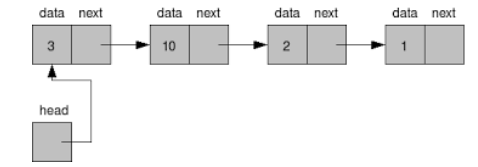
\includegraphics[width = 0.5\textwidth]{figs/linked-lists.png}
\end{figure}

\subsubsection{Árboles}
Los árboles contienen nodos de datos organizados de forma jerárquica con un único nodo raíz y los demás tienen un padre y quizás hijos.

\begin{figure}[htbp]
\centering
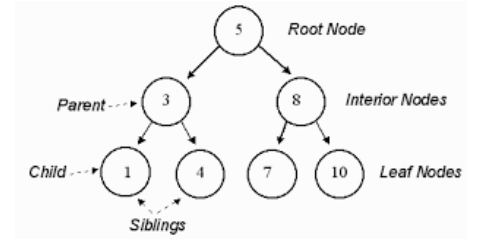
\includegraphics[width = 0.5\textwidth]{figs/tree-datastructure.png}
\end{figure}

\subsubsection{Grafos}
Los grafos están compuestos por nodos o vértices conectados por edges. Posiblemente es la estructura de datos más general: puede representar mapas de carreteras, redes sociales, interacciones de proteínas, etc.

\begin{figure}[htbp]
\centering
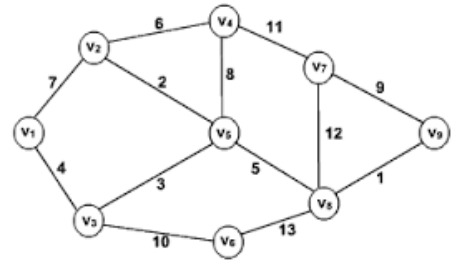
\includegraphics[width = 0.5\textwidth]{figs/graph-datastructure.png}
\end{figure}

\section{Diseño de algoritmos}
La escritura de algoritmos (y la programación en general) suele hacerse ad hoc. Es un acto creativo: debe seguir las reglas de programación pero también requiere imaginación, creatividad y experiencia. Lo mismo ocurre con la escritura ordinaria, ya que no podemos llenar una página vacía sólo con reglas gramaticales. La programación también requiere trabajo duro, mucha práctica y, además, bastante lectura de algoritmos. A veces podemos aprovechar las técnicas generales de diseño derivadas de una larga experiencia en resolución de problemas y análisis de algoritmos. No pueden aplicarse como reglas empíricas automáticas, pero pueden tener un amplio rango de aplicabilidad. Consideraremos tres: \textbf{algoritmos codiciosos}, \textbf{algoritmos de divide y vencerás} (también conocidos como \textbf{recursivos}) y \textbf{programación dinámica}.

\subsection{El problema del cambio - algoritmo codicioso}
Supongamos que tenemos trabajo como cajero y nuestros clientes quieren cambio en el menor número de monedas posible. ¿Cómo podemos proceder? La idea más sencilla: dar a cada paso la moneda más grande y más pequeña que la cantidad que queda por cambiar. Ejemplo: ¿cómo dar cambio de 3,44 euros? Fácil: una moneda de 2 euros, una moneda de 1 euro, dos monedas de 20 céntimos, dos monedas de 2 céntimos. Hay que escribir el algoritmo pero la idea general es codiciosa: Intentamos minimizar \textbf{globalmente} el número total de monedas, pero lo hacemos \textbf{localmente} usando en cada paso la moneda más grande posible para minimizar la cantidad que queda por cambiar.

Suponiendo que trabajamos con monedas/billetes de 1, 2, 5, 10, 20, 50, 100 y 200, queremos guardar el número de monedas/billetes de cada tipo a devolver en un diccionario:
\begin{lstlisting}
def change(c):
	assert c >= 0, "change for positive amounts only"
	l_coin_values = [1, 2, 5, 10, 20, 50, 100, 200]
	d_chainge = {}
	
	for coin in sorted(l_coin_values) [::-1]:
		d_change[coin] = c//coin
		c = c%coin
		
	return d_change
\end{lstlisting}

Aparentemente, esto funciona. Pero si debemos dar un cambio de 7 con monedas 1, 3, 4 o 5, la respuesta más eficiente solo requiere dos monedas, una de 4 y una de 3, pero este algoritmo cogería una de 5 y tendrá que dar dos monedas de 1. Esto ocurre bastante con algoritmos codiciosos: son muy naturales, pero pueden dar una respuesta equivocada. La forma de resolver esto sería con programación dinámica.

\subsection{Las torres de Hanoi - algoritmo recursivo}
Se nos da un conjunto de 64 discos de oro de diferentes tamaños apilados en la pila A en tamaños crecientes, y otras dos pilas vacías B, C. Queremos mover la primera pila a B un disco cada vez usando C como clavija auxiliar obedeciendo la regla de que ningún disco puede colocarse encima de otro disco más pequeño. Esto es fácil para 2 discos, no muy difícil para 3, pero para 4 la dificultad aumenta. 

Se puede obtener una solución recursiva sencilla para N discos. Primero se mueven los primeros N-1 discos de la pila A a la C utilizando B como pila auxiliar. El disco restante se mueve de A a B. Los N-1 discos restantes se mueven de C a B usando A como pila auxiliar. 
\begin{lstlisting}
def hanoi(n_disks, a=1, b=2, c=3):
	assert n_disks > 0, "n_disks at least 1"
	
	if n_disks == 1:
		print("Move disk from %d to %d" % (a,b))
	else:
		hanoi(n_disks - 1, a, c, b)
		print("move disk from %d to %d" % (a,b))
		hanoi(n_disks - 1, c, b, a)
\end{lstlisting}

Con esto, hay que tener cuidado con los tiempos de ejecución incluso para n\_disks pequeños. De hecho, el problema general de Hanoi es extremadamente costoso incluso para un número moderado de discos.

Los algoritmos recursivos suelen derivar de una estrategia de «divide y vencerás»: Dividir un problema P en M subproblemas $P_m$, resolverlos por separado obteniendo soluciones $S_m$ y combinar estas soluciones en una solución S de P.

En el caso de las torres de Hanoi se pueden dividir dos subproblemas: P1 es el subproblema de mover N - 1 discos de A a C usando B, y P2 el subproblema de mover N - 1 discos de C a B usando A. Se pueden combinar los movimientos según el código de Python. Los algoritmos son eficientes si los subproblemas son sustancialmente más pequeños - pero esto no es el caso de Hanoi.

\section{Eficiencia de algoritmos}
En primer lugar, los algoritmos deben ser correctos, ya que un algoritmo rápido, pero erróneo, es inútil.  También es deseable que no requieran (mucha) memoria extra. La función \texttt{hanoi} cumple esto: sólo se usan sus parámetros. Algo a tener en cuenta en bioinformática, ya que los datos pueden ser muy grandes, es que también es muy deseable que los algoritmos sean lo más rápidos posible. Pero un algoritmo debe leer sus entradas, y si hay muchas y grandes, esto ralentizará el algoritmo. No obstante, los tiempos de ejecución deseables no deberían estar muy por encima del \textbf{mismo orden de magnitud que el tamaño de sus entradas}.

\subsection{Estimar tiempos de ejecución}
En primer lugar, no se miden solo los tiempos reales, ya que dependen del lenguaje, la máquina, el programador y, por supuesto, las entradas. Por tanto, dependen demasiado del contexto para permitir generalizaciones significativas. En su lugar, hay que centrarse en \textbf{tiempos abstractos} medidos contando las \textbf{operaciones clave} que el algoritmo realiza en una entrada dada. Para los algoritmos iterativos, normalmente se busca la operación clave en el bucle más interno. Contando cuántas veces se realizan estas operaciones clave se obtiene una buena estimación del tiempo que tardarán los algoritmos. De esta forma, el coste del algoritmo de cambio viene dado por la longitud de la lista de monedas.

El análisis de algoritmos recursivos es (mucho) más difícil. Para Hanoi, la operación clave puede ser \texttt{print("move disk from \%d to \%d" \% (a, b))}, pero aunque aparece explícitamente en el código, también tiene lugar dentro de las llamadas recursivas. Esto da lugar a estimaciones recurrentes del coste de los algoritmos recursivos que a menudo son difíciles de escribir y resolver. Se pueden desarrollar algunas estrategias generales en algoritmos mucho más sencillos basados en bucles. 

\subsection{Multiplicación de matrices}
Un algoritmo muy conocido y relativamente costoso es $c_{i,j} = \sum^n_{k=1} a_{i,k}b_{k,j}$. Un código de Python simple y malo que describe esto es el siguiente:
\begin{lstlisting}
def matrix_multiplication(m_1, m_2):
	n_rows, n_interm, n_columns = m_1.shape[0], m_2.shape[0], m_2.shape[1]
	m_product = np.zeros( (n_rows, n_columns) )
	
	for p in range(n_rows):
		for q in range(n_columns):
			for r in range(n_interm):
				m_product[p, q] += m_1[p, r] * m_2[r, q]
				
	return m_product
\end{lstlisting}

Aquí, la operación clave es \texttt{m\_1[p, r] * m\_2[r, q]}. Asumiendo matrices cuadradas con N filas y columnas, esta operación clave se repite $N \times N \times N = N^3$, lo cual es sustancialmente más grande que el tamaño del problema $N^2 + N^2 = 2N^2$.

%04/02 
\subsection{Búsqueda lineal}
Para buscar una clave en una lista, lo más sencillo es comparar la clave con todos los elementos de la lista hasta que se encuentre. 
\begin{lstlisting}
def linear_search(key, l_ints):
	for i, val in enumerate(l_ints):
		if val == key:
			return i
				
	return None
\end{lstlisting}

En este caso, la operación clave es \texttt{if val == key}. Encontrar la clave que esté en \texttt{l\_ints[0]}, solo se requiere una operación, pero para \texttt{l\_ints[-1]}, se requieren \texttt{N = len(l\_ints)} operaciones, al igual que si la clave no se encuentra en la lista.

\subsection{Notación o, O y $\Theta$}
Dado un algoritmo, y sabiendo la operación básica, hay una función que calcula el coste de dicha operación. La multiplicación de matrices tiene un coste $f_{MM} (N) = N^3$, y la búsqueda lineal $f_{LS}(N) = N$. Por tanto, se pueden comparar dos algoritmos mediante la comparación de su función de coste.  

Suponemos que las funciones de coste son positivas y crecientes (así deberían ser los tiempos de ejecución abstractos de los algoritmos)

Se dice que $f = o(g)$ si ambas son positivas en el tiempo ($\frac{f(N)}{g(N)} \rightarrow 0$), y el crecimiento de $f$ es considerablemente menor que el de $g$.

Además, $f = O(g)$ si encontramos una constante C de un entero N que depende de C de manera que $f(N) \leq Cg(N)$ siempre que $N \geq N_C$. De esta forma, $g$ será eventualmente mayor que $f$ con la ayuda de $C$.

Finalmente, $f = \Theta(g)$ si $f = O(g)$ y $g = O(f)$. 

En resumen, y de manera informal, podemos decir:
\begin{itemize}
\item $f < g$ cuando $f = o(g)$
\item $f \leq g$ cuando $f = O(g)$
\item $f \approx g$ cuando $f = \Theta(g)$ y, por tanto, $g = \Theta(f)$
\end{itemize}

Por ejemplo, antes definimos unas funciones con coste $N^2$ y $N^3$. Al hacer $\frac{N^2}{N^3} = \frac{1}{N}$, tendiendo N a infinito, el resultado es 0, por lo que $N^2 = o(N^3)$. Además, como $N^2 \leq 1 \cdot N^3$, entonces también $N^2 = O(N^3)$, pero esto es menos preciso.

\subsection{Complejidad de un algoritmo}
A partir de un algoritmo A con un input I, se puede medir el tiempo de ejecución abstracto de la siguiente forma:
\begin{itemize}
\item Podemos identificar la operación clave en A y estimar su trabajo abstracto en I siguiendo el número $n_A(I)$ de veces que A se ejecuta en I.
\item Se puede asignar un tamaño N al input I
\item Podemos encontrar una función $f_A(N)$ de forma que $n_A(I) = O(f_A(N))$
\end{itemize}
En algunos casos, esto se puede refinar a $n_A(I) = \Theta(f_A(N))$. Por tanto, $f_A(N)$ da la complejidad de A sobre las entradas de tamaño N. Para el problema de Hanoi, tenemos $n_{Hanoi}(N) = 2^N - 1$. En las búsquedas lineales, aquellas búsquedas exitosas son $n^e_{LS}(N) \leq N$, pero también puede darse $n^e_{LS}(N) = 1$, por lo que el peor escenario de la búsqueda lineal es $W(N) = N$, ya que siempre $n_{LS}(k, l_ints) \leq N$.

\subsection{De tiempos abstractos a tiempos reales}
En Python, está el comando \texttt{\%timeit} que permite la estimación de tiempos de ejecución en el caso de funciones simples. 
\begin{lstlisting}
a = np.ones((100, 100))
b = np.eye(100)
%timeit -n 10 -r 1 matrix_multiplication(a, b)
\end{lstlisting}
Si \texttt{timeit} nos devuelve 1s (para 100 elementos), en el caso de matrices de 500 podemos esperar $500 = 5 \times 100, 500^3 = 125 \times 100^3$, es decir, 125 segundos. Esto no es muy preciso, pero sirve para una estimación. Hay que tener en cuenta que librerías grandes como \texttt{numpy} o \texttt{pandas} utilizan C o C++ para el código compilado al ser más rápido.
%04/02 - José Dorronsoro
\chapter{Programación dinámica}
\section{Revisando el problema del cambio}
Volvemos al problema de devolver el cambio de una cantidad de dinero. El algoritmo codicioso no siempre llegaba a la solución más óptima en cuanto a menor número de monedas devueltas. 
En este caso, el truco está en descomponer el problema en subproblemas y crear una fórmula para ir de un subproblema al siguiente.

Suponiendo que debemos dar un cambio C y tenemos las monedas $v_1 = 1, \ldots v_n$, entonces $n(i, c)$ es el número mínimo de monedas a cambiar utilizando solo las primeras $i$ monedas. Lo que queremos es $n(N, C)$, que se obtiene del subproblema $n(i, c)$. Además:
$$n(i,0) = 0$$
$$n(1,c) = c$$

Con esto, se puede rellenar una matriz con las monedas como filas y el posible cambio como columna. Para rellenar la posición $n(i,c)$:
\begin{itemize}
\item Si la moneda $i$ no entra en el cambio: $n(i - 1, c)$
\item Si la moneda $i$ sí entra en el cambio: $1 + n(i, c - v_i)$
\end{itemize}

\subsection{El algoritmo del cambio en programación dinámica}
De esta forma, llegamos a
$$n(i, c) = min{n(i - 1, c), 1 + n(i, c - v_i)}$$
con un coste $O(1)$.

En el problema, queríamos dar un cambio de 7 con monedas 1, 3, 4 y 5: $n(4, 7)$ Para ello, tenemos una tabla con las filas 1, 3, 4 y 5 y las columnas 0 1 2 3 4 5 6 7. La primera fila, con la moneda de 1, se rellena con el valor del cambio que hay que dar. Para la fila del 3, los valores de las columnas 0 1 y 2 se mantienen como la fila anterior, ya que no se puede utilizar esta moneda para un cambio menor a su valor. A partir del valor de la moneda, se debe retroceder ese valor en número de columnas y sumarle 1. Ese valor hay que compararlo con el de la celda justamente superior, y ver el valor mínimo, el cual se mantiene. Siguiendo esta lógica, llegamos a que el número de monedas mínimo para este problema son 2.

\begin{figure}[h]
\centering
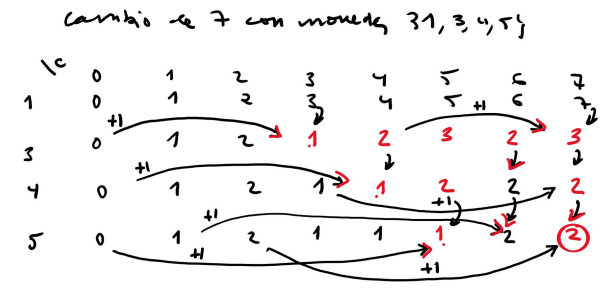
\includegraphics[width = 0.7\textwidth]{figs/dp-cambio.png}
\end{figure}

En este caso, hemos calculado $7 (c) \times 4 (n) = 28$ veces. El coste de un algoritmo sin bucles es constante: $f(n) = 1$. Por tanto, en este caso el coste es $28 \times O(1)$, y de forma general:
$$N \times C \times O(1) = O(N \times C) = O(N \times 2^{logC})$$
siendo $2^{logC}$ el logaritmo binario de C (los bits en los que se puede codificar).

\section{Algoritmos de cadenas en programación dinámica}
Para un informático, una secuencia biológica son cadenas de texto.
Teniendo dos cadenas, para transformar una en la otra, se puede:
\begin{itemize}
\item Cambiar un caracter por otro
\item Insertar un caracter
\item Borrar un caracter
\end{itemize}
Insertar un caracter en una cadena es equivalente a borrar un caracter en la otra. Además, queremos mantener una cadena constante y modificar solo la otra. 

La \textbf{distancia de edición} entre dos cadenas es el número mínimo de de operaciones de edición que se deben hacer para convertir una en la otra. 

Dados los strings S y T con M y N número de caracteres respectivamente,se consideran los substrings  
$$S_i = [s_1, \ldots s_i]$$
$$T_i = [t_1, \ldots t_j]$$

Así, $d_{i,j}$ es la distancia de edición entre $S_i$ y $T_i$. Si $s_i = t_j$, entonces $d_{i,j} = d_{i-1, j-1}$, ya que la diferencia se encuentra antes. Si $s_i \neq t_j$, hay tres opciones:
\begin{itemize}
\item Cambiar $t_j$ por $s_i$; entonces $d_{i,j} = 1 + d_{i-1, j-1}$
\item Borrar $t_j$ de $T_j$; entonces $d_{i,j} = 1 + d_{i, j-1}$
\item Borrar $s_i$ de $S_i$; entonces $d_{i,j} = 1 + d_{i-1, j}$
\end{itemize}
De estas tres opciones, se calculan todas y nos quedamos con el mínimo.

\subsection{Rellenar la matriz}
Tenemos una matriz con M filas y N columnas. Esto se multiplica por lo que cuesta calcular cada elemento, O(1): $O(M \times N)$. Esto es caro en tiempo y en memoria. 

Finalmente, tenemos las siguientes ecuaciones para el problema de la distancia de edición:
$$d_{i,j} = \begin{cases}
d_{i-1, j-1} & \text{cuando} s_i = t_j \\
1 + min {d_{i-1, j-1}, d_{i, j-1}, d_{i-1, j}} & \text{cuando} s_i \neq t_j
\end{cases} $$

Ejemplo: encontrar la distancia de edición entre \texttt{biscuit} y \texttt{suitcase}.
\begin{figure}[h]
\centering
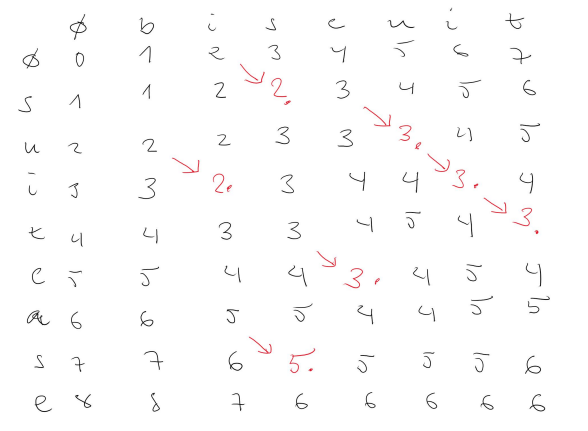
\includegraphics[width = 0.6\textwidth]{figs/edit-distance-ex.png}
\end{figure}

No obstante, en biología, se asignan costes a cambiar y a borrar diferentes dependiendo del caso.

\chapter{Resumen complejidad algorítmica}
\begin{table}[h]
\centering
\begin{tabular}{l l }
\multicolumn{2}{c}{O: Peor caso} \\ \hline
$O(1)$ & \texttt{def constante(arr): return arr[0]} \\ 
$O(n)$ & \texttt{for x in arr: print(x)} \\ 
$O(n^k)$ & \texttt{for i in range(n):} \\ 
 & \texttt{\ \ for j in range(n): print(arr[i], arr[j])} \\ 
$O(\log n)$ & \texttt{while n > 1: n //= 2} \\ 
$O(\log \log n)$ & \texttt{while n > 2: n = log2(n)}  \\ 
$O(n \log n)$ & \texttt{merge\_sort(arr)} \\ 
\end{tabular}
\end{table}

\begin{table}[h]
\centering
\begin{tabular}{l l }
\multicolumn{2}{c}{o: Límite superior no ajustado} \\ \hline
$o(1)$ & No aplica (es constante) \\ 
$o(n)$ & \texttt{for i in range(sqrt(n)): print(i)}\\ 
$o(n^k)$ & \texttt{for i in range(n):} \\ 
 & \texttt{\ \ for j in range(log(n)): print(i, j)} \\ 
$o(\log n)$ & \texttt{while n > 1: n = sqrt(n)}  \\ 
$o(\log \log n)$ & \texttt{while n > 2: n = log2(log2(n))}  \\ 
\end{tabular}
\end{table}

\begin{table}[h]
\centering
\begin{tabular}{l l }
 \multicolumn{2}{c}{$\Theta$: Límite ajustado} \\ \hline
$\Theta(1)$ & \texttt{def constante(arr): return arr[0]} \\ 
$\Theta(n)$ & \texttt{for x in arr: print(x)} \\ 
$\Theta(n^k)$ & \texttt{for i in range(n):} \\ 
& \texttt{\ \ for j in range(n): print(arr[i], arr[j])} \\ 
$\Theta (\log n)$ & \texttt{while n > 1: n //= 2} \\ 
$\Theta (\log \log n)$ & \texttt{while n > 2: n = log2(n)} \\ 
$\Theta(n \log n)$ & \texttt{merge\_sort(arr)} \\ 
\end{tabular}
\end{table}

\end{document}
